\section{Background}
In this section, we give some needed background on floating-point arithmetic.
% \subsection{SMACK}
% \begin{figure}[tb]
%   \centering
%   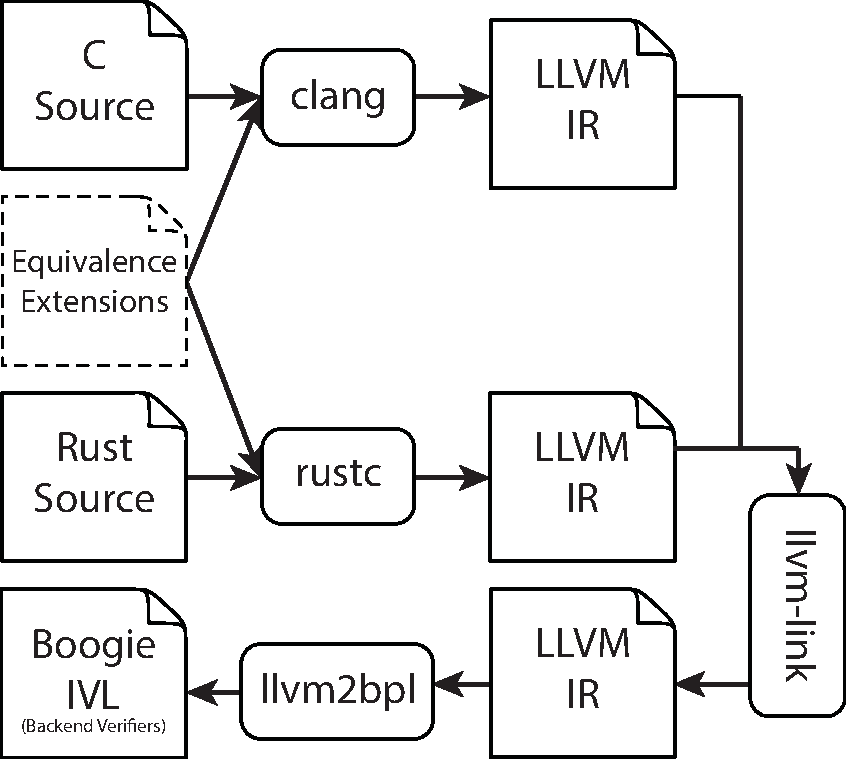
\includegraphics[width=0.92\textwidth]{chap4/fig/SmackEquiv.pdf}
%   \caption{Toolflow of SMACK.}
%   \label{fig:toolflow}
% \end{figure}

% SMACK~\cite{smack} is a software verification toolchain that translates
% LLVM IR code into Boogie intermediate verification language~\cite{boogie}, which
% is in turn verified using back-end Boogie verifiers such as the
% Boogie~\cite{boogie} verifier and the Corral~\cite{corral} verifier.
% %
% SMACK has been predominantly used to verify LLVM IR programs produced by the
% Clang C compiler.
% %
% SMACK has been extended to support additional programming languages, in
% particular the Rust programming language~\cite{2018_atva_bhr}.
% %
% We exploit this ability of SMACK to work with multiple languages together in
% this work.


% \Cref{fig:toolflow} shows the toolflow of SMACK, which works as follows:
% %
% \begin{enumerate}
% \item The SMACK top-level script automates the entire toolflow. It determines
%   which compilers to invoke and flags to use for program compilation. In the case
%   of C programs, it invokes Clang to generate LLVM IR code, while including
%   SMACK's C language models. The models specify the semantics of common C
%   library functions such as malloc, free, and string operations.
% \item For Rust programs, SMACK invokes the Rust compiler~\cite{rust14}
%   and links in its own Rust models. This includes Rust language support for
%   verification functionality.
% \item The common models file is then linked with the generated LLVM IR files to
%   provide basic verification capabilities. This includes
%   modeling dynamic memory allocation, supporting assertions and
%   assumptions, and generating nondeterministic values.
% \item The core \textsc{llvm2bpl} component takes an LLVM IR file as input, and
%   produces Boogie intermediate verification language (IVL) code that captures the semantics of LLVM IR instructions;
%   it outputs a Boogie file for verification.
% \item Finally, the Boogie or Corral back-end verifiers are invoked on the
%   generated Boogie file. We use Z3~\cite{z3} and CVC5~\cite{cvc5} as their SMT
%   solvers.
% \end{enumerate}

% In this work, we use Corral and Boogie in their bounded verification modes,
% meaning that loops are unrolled and recursive functions are expanded up to a
% certain user-provided bound.

\subsection{Floating-Point Arithmetic}
Floating-point arithmetic is an approximation of real-arithmetic using
fixed-sized representations.
%
Because floating-point numbers have a fixed size, operations involving them may
involve rounding to keep the resulting number's size fixed.
%
Rounding means some familiar algebraic identities, such as associativity of both
addition and multiplication, do not hold for these operations on floating-point
numbers.
%
There is a finite range of values that floating-point numbers can represent,
there are positive and negative infinity values to represent numbers outside
this range.
%
A final class of floating-point values is the \textit{NaN} (Not a Number) values
which represent the results of invalid computations such as division by 0.
%
NaN values propagate, e.g., adding a NaN with another value produces a NaN, to
allow these faulty calculations to be detected when convenient.
%
A notable property of NaN values is that they are not equal to any other
floating-point value, including other NaN values.
%
In the SMT theory of floating-points, there is one NaN value that is not
comparable to any other value.
